\begin{frame}{}
    \LARGE NLP: \textbf{Recurrent Neural Networks (RNNs)}
\end{frame}

\begin{frame}{Limitations of Traditional Approaches}
    \begin{itemize}
        \item \textbf{Bag-of-Words and n-gram models:}
        \begin{itemize}
            \item Ignore word order and long-range dependencies.
            \item Fixed-size context window limits understanding of sequence.
            \item Consume more memory and computational resources for larger contexts.
        \end{itemize}
        \item \textbf{Feedforward Neural Networks:}
        \begin{itemize}
            \item Cannot handle variable-length input sequences.
            \item Lack memory of previous inputs.
        \end{itemize}
    \end{itemize}
\end{frame}

\begin{frame}[t]{How RNNs Helps}
    \begin{columns}
        \begin{column}{0.6\textwidth}
            \centering
            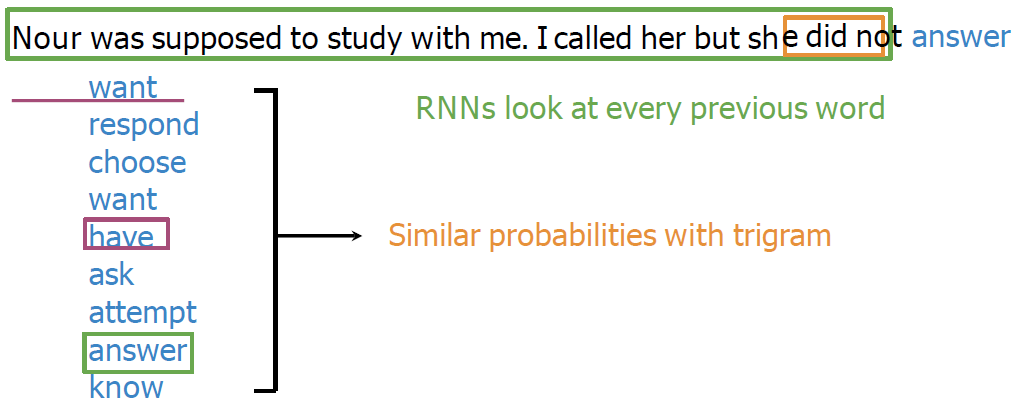
\includegraphics[width=1.1\linewidth]{images/nlp/rnn-advantage.png}  
        \end{column}
        \begin{column}{0.4\textwidth}
            \begin{itemize}
                \setlength{\itemsep}{1.5em}
                \item Designed to process sequential data of arbitrary length.
                \item Maintain a hidden state to capture context and dependencies over time.
                \item Better suited for tasks like language modeling, translation, and sequence prediction.
            \end{itemize}
        \end{column}
    \end{columns}
\end{frame}

\begin{frame}{RNNs Basic}
    \begin{figure}
        \centering
        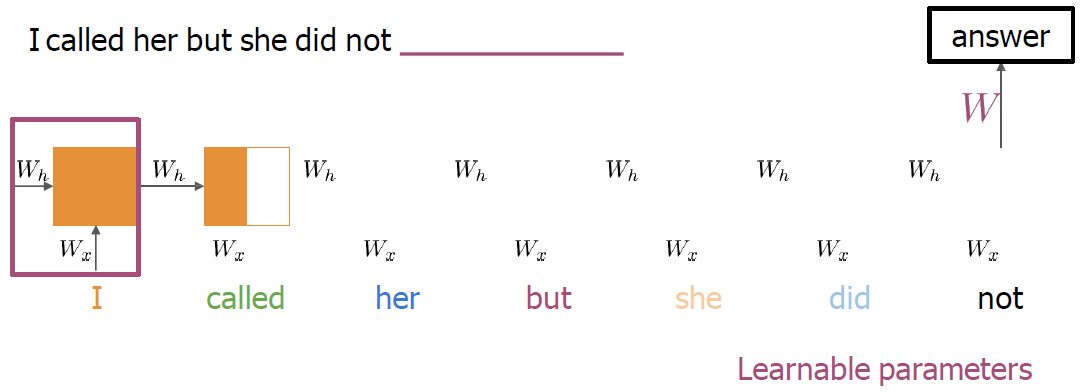
\includegraphics[width=\linewidth]{images/nlp/rnn-basic.png}
    \end{figure}

    \begin{itemize}
        \item RNNs model relationships among distant words in a sequence.
        \item Many computations in RNNs share parameters across time steps, enabling efficient learning and generalization.
    \end{itemize}
\end{frame}

\begin{frame}{One to One}
    \begin{figure}
        \centering
        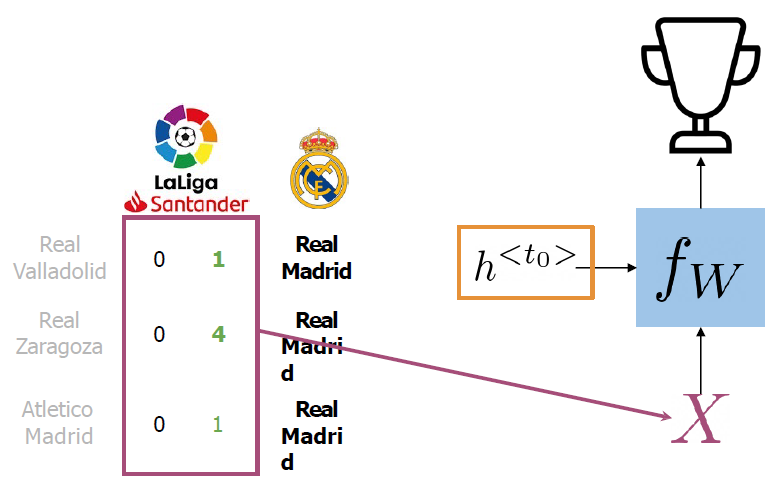
\includegraphics[width=\linewidth, height=0.9\textheight,keepaspectratio]{images/nlp/rnn-one2one.png}
    \end{figure}
\end{frame}

\begin{frame}{One to Many}
    \begin{figure}
        \centering
        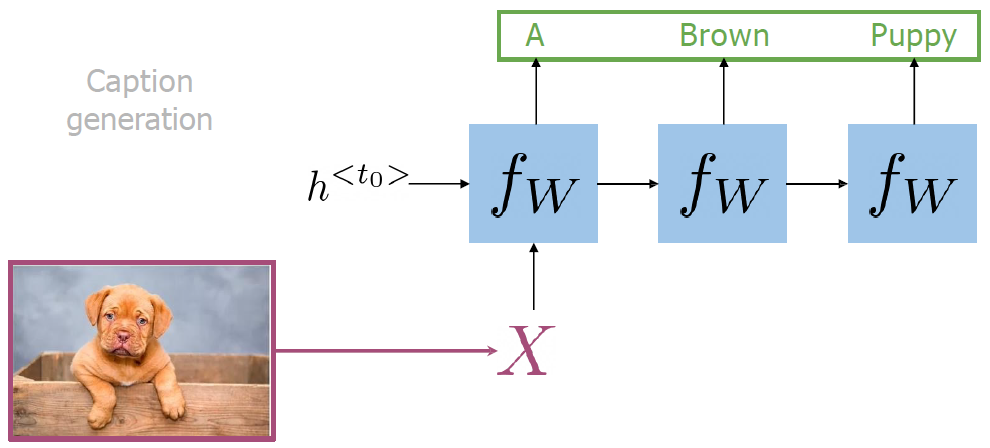
\includegraphics[width=\linewidth, height=0.9\textheight,keepaspectratio]{images/nlp/rnn-one2many.png}
    \end{figure}
\end{frame}

\begin{frame}{Many to One}
    \begin{figure}
        \centering
        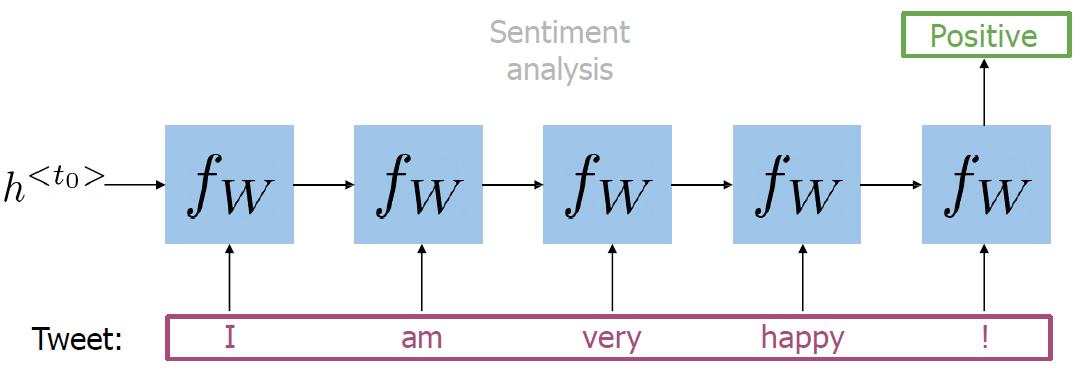
\includegraphics[width=\linewidth, height=0.9\textheight,keepaspectratio]{images/nlp/rnn-many2one.png}
    \end{figure}
\end{frame}
\begin{frame}{Many to Many}
    \begin{figure}
        \centering
        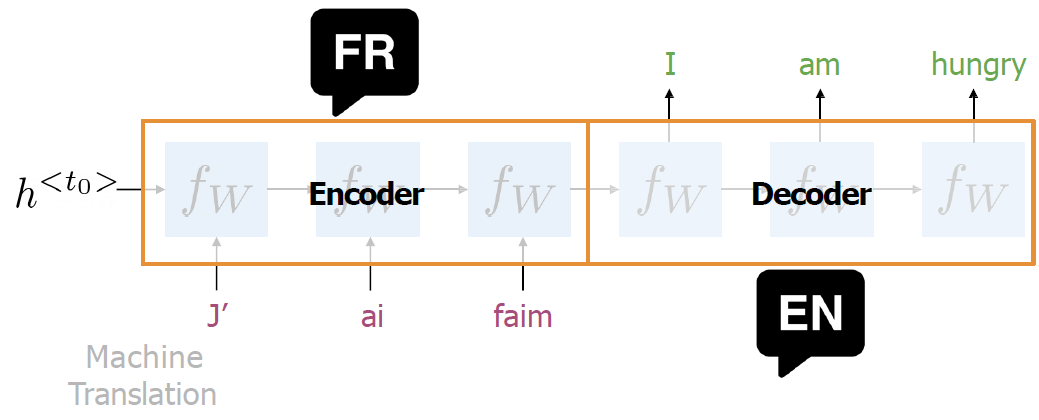
\includegraphics[width=\linewidth, height=0.9\textheight,keepaspectratio]{images/nlp/rnn-many2many.png}
    \end{figure}
\end{frame}

\begin{frame}{Math in Simple RNNs}
    \begin{itemize}
        \item \textbf{Propagation through time:}
        \begin{align*}
            h_t &= \sigma(W_{xh} x_t + W_{hh} h_{t-1} + b_h)
        \end{align*}
        where $x_t$ is the input at time $t$, $h_{t-1}$ is the previous hidden state, $W_{xh}$ and $W_{hh}$ are weight matrices, $b_h$ is the bias, and $\sigma$ is an activation function (e.g., $\tanh$ or $\text{ReLU}$).
        \item \textbf{Making predictions:}
        \begin{align*}
            y_t &= \phi(W_{hy} h_t + b_y)
        \end{align*}
        where $W_{hy}$ is the output weight matrix, $b_y$ is the output bias, and $\phi$ is an activation function (e.g., softmax for classification).
    \end{itemize}
    \vspace{1em}
    \textbf{Key idea:} The hidden state $h_t$ acts as memory, allowing information to flow from previous time steps to influence current predictions.
\end{frame}

\begin{frame}[allowframebreaks]{A Vanilla RNN}
    \begin{figure}
        \centering
        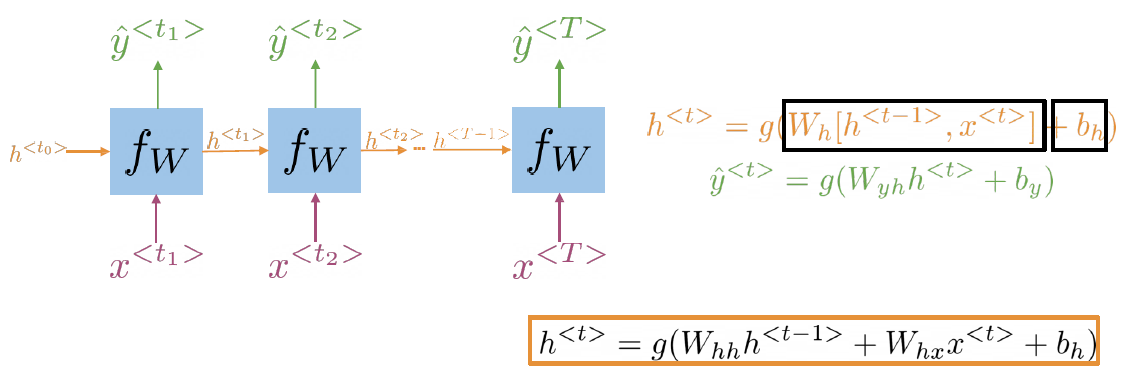
\includegraphics[width=\linewidth, height=0.9\textheight,keepaspectratio]{images/nlp/rnn-vanilla.png}
    \end{figure}

    \framebreak

    \begin{figure}
        \centering
        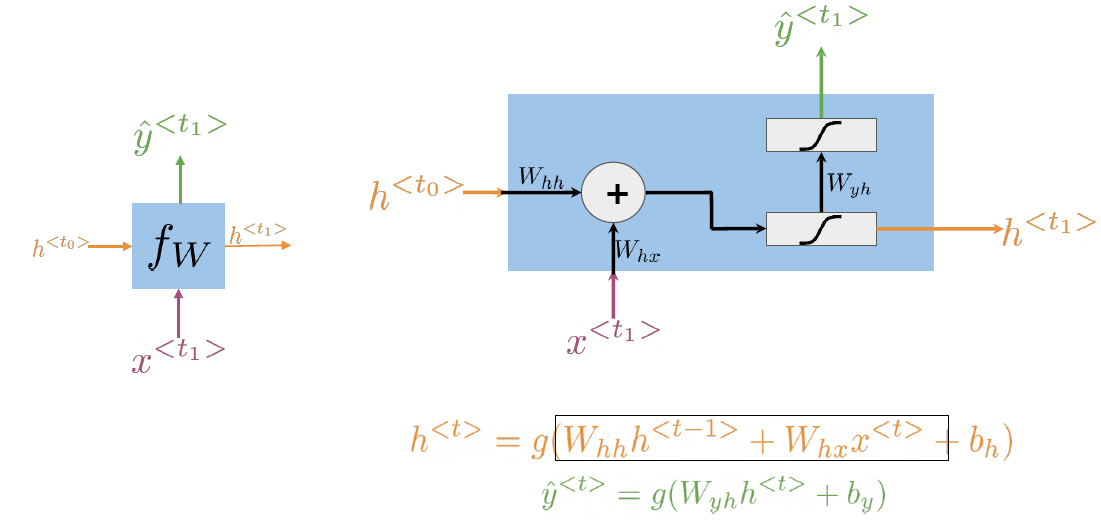
\includegraphics[width=\linewidth, height=0.9\textheight,keepaspectratio]{images/nlp/rnn-vanilla-2.png}
    \end{figure}

    \begin{itemize}
        \item Hidden states propagate information through time.
        \item Basic recurrent units have two inputs at each time: $x^{\langle t \rangle}$ (current input) and $h^{\langle t-1 \rangle}$ (previous hidden state).
    \end{itemize}
\end{frame}

\begin{frame}{Cross Entropy Loss}
    \begin{figure}
        \centering
        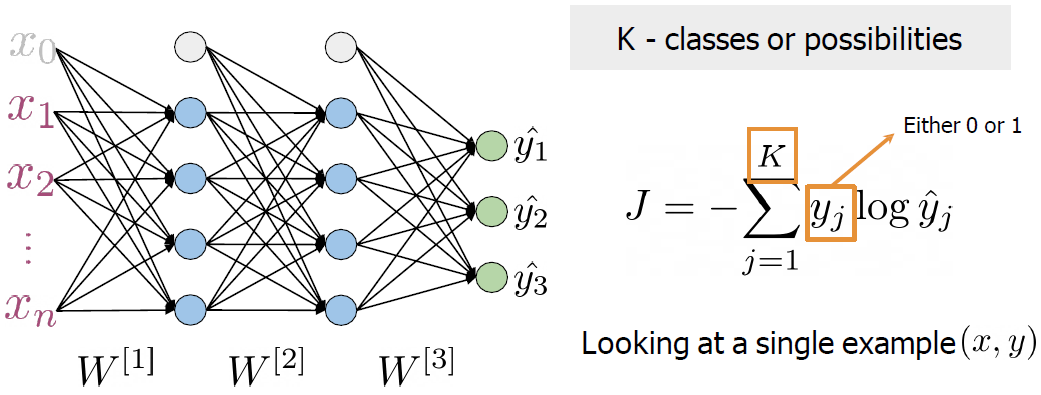
\includegraphics[width=\linewidth, height=0.9\textheight,keepaspectratio]{images/nlp/rnn-cross-entropy.png}
    \end{figure}
\end{frame}

\begin{frame}{Cross Entropy Loss for RNNs}
    \begin{figure}
        \centering
        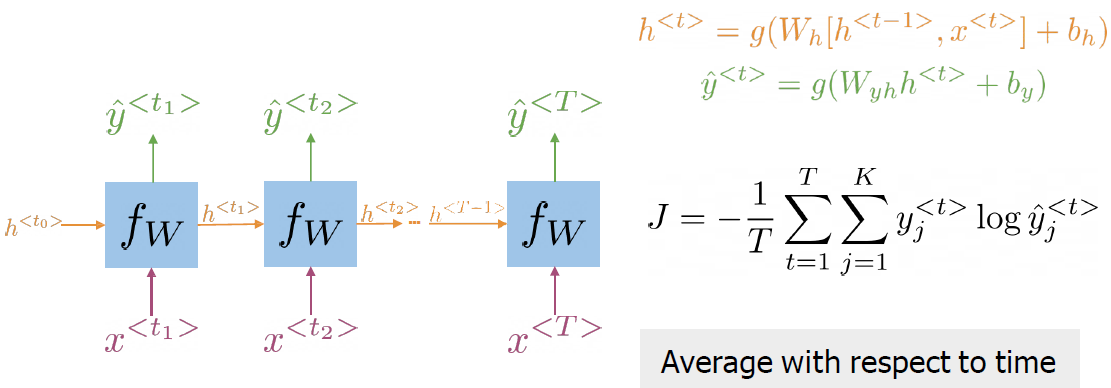
\includegraphics[width=\linewidth, height=0.9\textheight,keepaspectratio]{images/nlp/rnn-cross-entropy-loss.png}
    \end{figure}
    For RNNs the loss function is just an average through time!
\end{frame}